    % File: 2_co_so_ly_thuyet/2.3_chuan_giao_tiep.tex

    \subsection{Chuẩn giao tiếp AMBA AXI4}
    AMBA (Advanced Microcontroller Bus Architecture) là tiêu chuẩn kết nối trên chip (On-Chip Interconnect) phổ biến nhất hiện nay, được phát triển bởi ARM. Trong đó, giao thức AXI (Advanced eXtensible Interface) là chuẩn giao tiếp hiệu năng cao, được thiết kế cho các hệ thống SoC yêu cầu băng thông lớn và độ trễ thấp.

    Phiên bản AXI4 (được giới thiệu trong AMBA 4.0) hỗ trợ các tính năng vượt trội so với các thế hệ trước:
    \begin{itemize}
        \item Tách biệt hoàn toàn pha địa chỉ/điều khiển và pha dữ liệu.
        \item Hỗ trợ giao dịch dữ liệu không thẳng hàng (Unaligned data transfers).
        \item Cho phép phát hành nhiều địa chỉ chờ (Outstanding addresses) trước khi dữ liệu hoàn tất.
        \item Hỗ trợ hoàn thành giao dịch không theo thứ tự (Out-of-order completion) thông qua ID.
    \end{itemize}

    \begin{figure}[H]
        \centering
        \includegraphics[width=0.5\linewidth]{2_co_so_ly_thuyet/image/axi.png} 
        \caption{a. Tổng quan giao thức AXI4}
        \label{fig:axi_channels}
    \end{figure}

    \begin{figure}[H]
        \centering
        \includegraphics[width=0.9\linewidth]{2_co_so_ly_thuyet/image/axi2.png} 
        \caption{b. Tổng quan giao thức AXI4}
        \label{fig:axi_channels}
    \end{figure}



    \subsubsection{Kiến trúc 5 kênh độc lập (Channel Architecture)}
    AXI chia nhỏ một giao dịch truyền thông thành 5 kênh riêng biệt hoạt động song song. Kiến trúc này cho phép đường truyền dữ liệu hai chiều (Full-duplex), nghĩa là Master có thể ghi dữ liệu vào Slave trong khi đang đọc dữ liệu từ Slave khác.

    \begin{figure}[H]
        \centering
        \includegraphics[width=0.9\linewidth]{2_co_so_ly_thuyet/image/axichannel.png} 
        \caption{Mô hình 5 kênh giao tiếp của AXI4}
        \label{fig:axi_channels}
    \end{figure}

    Năm kênh tín hiệu bao gồm:
    \begin{enumerate}
        \item \textbf{Write Address Channel (AW):} Master gửi địa chỉ bắt đầu và thông tin điều khiển (loại burst, độ dài) cho giao dịch ghi. Các tín hiệu bắt đầu bằng \texttt{AW...} (ví dụ: \texttt{AWADDR}, \texttt{AWVALID}).
        \item \textbf{Write Data Channel (W):} Master truyền dữ liệu thực tế tới Slave. Kênh này hỗ trợ tín hiệu \texttt{WSTRB} (Strobe) để đánh dấu các byte hợp lệ trong một word (hỗ trợ ghi từng byte). Các tín hiệu bắt đầu bằng \texttt{W...}.
        \item \textbf{Write Response Channel (B):} Slave gửi phản hồi trạng thái (OKAY, ERROR) cho Master sau khi toàn bộ dữ liệu đã được ghi thành công. Tín hiệu bắt đầu bằng \texttt{B...}.
        \item \textbf{Read Address Channel (AR):} Master gửi địa chỉ bắt đầu cho giao dịch đọc. Tín hiệu bắt đầu bằng \texttt{AR...}.
        \item \textbf{Read Data Channel (R):} Slave trả về dữ liệu yêu cầu cùng với trạng thái đọc. Tín hiệu bắt đầu bằng \texttt{R...}.
    \end{enumerate}

    \subsubsection{Cơ chế bắt tay (Handshake Mechanism)}
    Toàn bộ 5 kênh AXI đều sử dụng chung một cơ chế bắt tay hai chiều \texttt{VALID/READY} để điều khiển luồng dữ liệu:
    \begin{itemize}
        \item \textbf{VALID (từ Bên gửi):} Báo hiệu rằng dữ liệu hoặc địa chỉ trên đường truyền đã hợp lệ và ổn định.
        \item \textbf{READY (từ Bên nhận):} Báo hiệu rằng bên nhận đã sẵn sàng chấp nhận dữ liệu mới.
    \end{itemize}

    \begin{figure}[H]
        \centering
        \includegraphics[width=0.9\linewidth]{2_co_so_ly_thuyet/image/battay.png} 
        \caption{Cơ chế bắt tay VALID/READY trong AXI}
        \label{fig:axi_handshake}
    \end{figure}

    Giao dịch chỉ thực sự diễn ra tại cạnh dương của xung nhịp khi và chỉ khi cả \texttt{VALID} và \texttt{READY} đều ở mức cao (High). Cơ chế này cho phép bên nhận có thể "kìm" (back-pressure) bên gửi nếu bộ đệm bị đầy, hoặc bên gửi có thể đợi chuẩn bị dữ liệu xong mới phát tín hiệu.

    Dựa trên cơ chế bắt tay này, chuẩn AXI định nghĩa hai cấp độ truyền tải dữ liệu cần phân biệt rõ:
    \begin{itemize}
        \item \textbf{Transfer (hoặc Beat):} Là một lần trao đổi dữ liệu đơn lẻ thành công (một lần bắt tay VALID/READY = 1). Trong một chuỗi dữ liệu (Burst), mỗi nhịp truyền một gói tin (ví dụ 32-bit) được gọi là một Transfer.
        
        \begin{figure}[H]
            \centering
            \includegraphics[width=0.9\linewidth]{2_co_so_ly_thuyet/image/transfer.png} 
            \caption{Minh họa một Transfer trong AXI}
            \label{fig:axi_handshake}
        \end{figure}

        \item \textbf{Transaction (Giao dịch):} Là một hoạt động đọc hoặc ghi hoàn chỉnh. Một Transaction bao gồm toàn bộ quá trình: gửi địa chỉ (Address Phase), truyền một hoặc nhiều dữ liệu (Data Phase - gồm nhiều Transfers) và nhận phản hồi (Response Phase).
        \begin{figure}[H]
            \centering
            \includegraphics[width=0.9\linewidth]{2_co_so_ly_thuyet/image/transaction.png} 
            \caption{Minh họa một Transaction trong AXI}
            \label{fig:axi_handshake}
        \end{figure}

    \end{itemize}

    % --- ĐOẠN BỔ SUNG VÀO SAU PHẦN TRANSFER/TRANSACTION ---% --- THAY THẾ CHO MỤC QUY TRÌNH GIAO DỊCH CŨ ---

    \subsubsection{Quy trình thực hiện giao dịch chi tiết (Transaction Steps)}
    Để đảm bảo toàn vẹn dữ liệu, chuẩn AXI quy định chặt chẽ về hướng đi của tín hiệu và trình tự bắt tay giữa Master và Slave. Dưới đây là mô tả chi tiết các tín hiệu tham gia vào hai loại giao dịch cơ bản.

    \textbf{1. Giao dịch Ghi (Write Transaction)} \\
    Quá trình ghi dữ liệu diễn ra qua 3 pha, sử dụng các kênh AW, W và B.

    \begin{figure}[H]
        \centering
        \includegraphics[width=0.9\linewidth]{2_co_so_ly_thuyet/image/write.png} 
        \caption{Giản đồ tín hiệu chi tiết của giao dịch Ghi}
        \label{fig:axi_write_trans}
    \end{figure}

    \begin{itemize}
        \item \textbf{Pha địa chỉ (Write Address Channel):}
        \begin{itemize}
            \item \textbf{Master $\rightarrow$ Slave:} Master đặt địa chỉ lên bus \texttt{AWADDR} và các thông tin điều khiển (Burst type, length) lên \texttt{AWLEN}, \texttt{AWSIZE}... sau đó xác lập tín hiệu \texttt{AWVALID = 1}.
            \item \textbf{Slave $\rightarrow$ Master:} Khi Slave sẵn sàng nhận địa chỉ, nó bật \texttt{AWREADY = 1}. Giao dịch địa chỉ hoàn tất.
        \end{itemize}
        
        \item \textbf{Pha dữ liệu (Write Data Channel):}
        \begin{itemize}
            \item \textbf{Master $\rightarrow$ Slave:} Master đưa dữ liệu lên bus \texttt{WDATA}. Nếu đây là gói cuối cùng trong Burst, Master bật tín hiệu \texttt{WLAST = 1}. Đồng thời, Master xác lập \texttt{WVALID = 1}.
            \item \textbf{Slave $\rightarrow$ Master:} Slave bật \texttt{WREADY = 1} để báo hiệu đã nhận gói dữ liệu đó. Quá trình lặp lại cho đến hết Burst.
        \end{itemize}

        \item \textbf{Pha phản hồi (Write Response Channel):}
        \begin{itemize}
            \item \textbf{Slave $\rightarrow$ Master:} Sau khi nhận đủ dữ liệu và hoàn tất việc ghi vào bộ nhớ, Slave gửi trạng thái (ví dụ: OKAY) qua bus \texttt{BRESP} và xác lập \texttt{BVALID = 1}.
            \item \textbf{Master $\rightarrow$ Slave:} Master xác nhận đã nhận được phản hồi bằng cách bật \texttt{BREADY = 1}. Kết thúc giao dịch.
        \end{itemize}
    \end{itemize}

    \textbf{2. Giao dịch Đọc (Read Transaction)} \\
    Quá trình đọc dữ liệu diễn ra qua 2 pha, sử dụng kênh AR và R.

    \begin{figure}[H]
        \centering
        \includegraphics[width=0.9\linewidth]{2_co_so_ly_thuyet/image/read.png} 
        \caption{Giản đồ tín hiệu chi tiết của giao dịch Đọc}
        \label{fig:axi_read_trans}
    \end{figure}

    \begin{itemize}
        \item \textbf{Pha địa chỉ (Read Address Channel):}
        \begin{itemize}
            \item \textbf{Master $\rightarrow$ Slave:} Master đặt địa chỉ cần đọc lên bus \texttt{ARADDR} cùng các tham số điều khiển, sau đó bật \texttt{ARVALID = 1}.
            \item \textbf{Slave $\rightarrow$ Master:} Slave chấp nhận địa chỉ bằng cách bật \texttt{ARREADY = 1}.
        \end{itemize}

        \item \textbf{Pha dữ liệu (Read Data Channel):}
        \begin{itemize}
            \item \textbf{Slave $\rightarrow$ Master:} Slave truy xuất dữ liệu và đưa lên bus \texttt{RDATA}. Nếu thành công, Slave gửi kèm trạng thái OKAY trên bus \texttt{RRESP}. Tại gói dữ liệu cuối cùng, Slave bật \texttt{RLAST = 1}. Tín hiệu \texttt{RVALID = 1} được xác lập khi dữ liệu trên bus là hợp lệ.
            \item \textbf{Master $\rightarrow$ Slave:} Master nhận dữ liệu bằng cách bật \texttt{RREADY = 1}.
        \end{itemize}
    \end{itemize}
    
    % --- HẾT PHẦN BỔ SUNG ---


    \subsubsection{Cấu trúc giao dịch Burst (Burst Transaction)}
    AXI là giao thức dựa trên Burst, nghĩa là chỉ cần gửi một địa chỉ khởi đầu, Master có thể truyền liên tiếp một chuỗi dữ liệu (tức là thực hiện một Transaction gồm nhiều Transfers). Các tham số chính điều khiển Burst bao gồm:

    \begin{itemize}
        \item \textbf{Burst Length (AxLEN):} Số lượng gói dữ liệu (beat/transfer) trong một burst. AXI4 hỗ trợ lên đến 256 beat cho kiểu INCR.
        \item \textbf{Burst Size (AxSIZE):} Số byte trong mỗi beat (ví dụ: 4 bytes cho hệ thống 32-bit).
        \item \textbf{Burst Type (AxBURST):} Xác định cách tính địa chỉ cho các beat tiếp theo:
        \begin{itemize}
            \item \textit{FIXED:} Địa chỉ giữ nguyên (dùng cho FIFO).
            \item \textit{INCR (Incrementing):} Địa chỉ tăng dần (dùng cho RAM). Đây là kiểu phổ biến nhất.
            \item \textit{WRAP:} Địa chỉ tăng đến giới hạn biên rồi quay vòng (dùng cho Cache Line fill).
        \end{itemize}
    \end{itemize}

    \subsubsection{Các biến thể giao thức trong thiết kế}
    Trong phiên bản AXI4, chuẩn AMBA định nghĩa thêm các biến thể rút gọn để phù hợp với từng mục đích sử dụng cụ thể:

    \textbf{1. Giao thức AXI4-Lite (AXI-Lite)} \\
    AXI4-Lite là một phiên bản rút gọn của AXI4, được thiết kế cho các giao tiếp điều khiển đơn giản, không yêu cầu truyền dữ liệu tốc độ cao (Burst transfer). Đặc điểm chính của AXI4-Lite bao gồm:
    \begin{itemize}
        \item Mỗi giao dịch chỉ truyền một gói dữ liệu đơn lẻ (Burst length = 1).
        \item Dữ liệu thường có độ rộng 32-bit hoặc 64-bit cố định.
        \item Đơn giản hóa logic điều khiển, giảm diện tích phần cứng.
    \end{itemize}
    Nhờ sự đơn giản này, AXI4-Lite thường được sử dụng làm giao diện cấu hình cho các thanh ghi điều khiển (Control Registers) bên trong các khối IP (Intellectual Property).

    \textbf{2. Giao thức AXI4-Stream (AXI-Stream)} \\
    AXI4-Stream được thiết kế chuyên biệt cho việc truyền tải các luồng dữ liệu liên tục tốc độ cao (Streaming data) mà không cần sử dụng địa chỉ. Khác với AXI4-Lite hay AXI4-Full (Memory Mapped), AXI4-Stream chỉ tập trung vào việc đẩy dữ liệu từ nguồn (Master) đến đích (Slave) nhanh nhất có thể.
    \begin{itemize}
        \item Không có kênh địa chỉ (Address Channel), giảm đáng kể số lượng dây tín hiệu.
        \item Hỗ trợ truyền dữ liệu liên tục không giới hạn độ dài Burst.
        \item Thích hợp cho dữ liệu video, âm thanh hoặc dữ liệu mạng nơ-ron (Feature maps).
    \end{itemize}

    \subsubsection{Áp dụng trong hệ thống đề tài}
    Trong khuôn khổ đồ án thiết kế SoC RISC-V tích hợp EdgeAI này, nhóm thực hiện áp dụng kết hợp cả hai chuẩn giao tiếp trên để tối ưu hóa hiệu năng và tài nguyên:

    \begin{itemize}
        \item \textbf{Sử dụng AXI4-Lite:} Đóng vai trò là kênh điều khiển (Control Plane). Vi xử lý PicoRV32 (Master) sẽ sử dụng AXI4-Lite để ghi vào các thanh ghi cấu hình của khối ngoại vi, khối Accelerator và DMA, thiết lập các thông số như kích thước ảnh, địa chỉ bộ nhớ và tín hiệu bắt đầu (Start).
        \item \textbf{Sử dụng AXI4-Stream:} Đóng vai trò là kênh dữ liệu (Data Plane). Dữ liệu hình ảnh từ Camera và các ma trận trọng số (Weights) sẽ được truyền trực tiếp từ DMA vào khối Accelerator thông qua AXI4-Stream. Việc loại bỏ overhead của kênh địa chỉ giúp tối đa hóa băng thông xử lý cho mạng CNN.
    \end{itemize}

    %%%%%%%%%%%%%%%%%%%%%%%%%%%%%%%%%%%%%%%%%%%%%
    \subsection{Giao thức truyền thông UART}

    UART (Universal Asynchronous Receiver-Transmitter) là một vi mạch phần cứng dùng để truyền tải dữ liệu nối tiếp giữa hai thiết bị. Khác với các giao thức đồng bộ như SPI hay I2C, UART hoạt động theo cơ chế bất đồng bộ (Asynchronous), nghĩa là không cần tín hiệu xung nhịp (Clock) chung để đồng bộ hóa việc truyền nhận giữa bên gửi và bên nhận.

    Trong các thiết kế SoC, UART thường được tích hợp như một khối ngoại vi (Peripheral) để phục vụ việc gỡ lỗi (Debug), in log hệ thống hoặc giao tiếp với máy tính.

    \subsubsection{Nguyên lý hoạt động}
    Giao thức UART truyền dữ liệu trên hai dây tín hiệu riêng biệt:
    \begin{itemize}
        \item \textbf{TX (Transmit):} Chân truyền dữ liệu đi.
        \item \textbf{RX (Receive):} Chân nhận dữ liệu về.
    \end{itemize}
    Để giao tiếp thành công, chân TX của thiết bị này phải được nối với chân RX của thiết bị kia và ngược lại. Quá trình truyền tin diễn ra bằng cách chuyển đổi dữ liệu song song (Parallel data) từ bus hệ thống thành luồng dữ liệu nối tiếp (Serial bit stream) tại phía phát, và khôi phục lại thành song song tại phía thu.
    
    \begin{figure}[H]
        \centering
        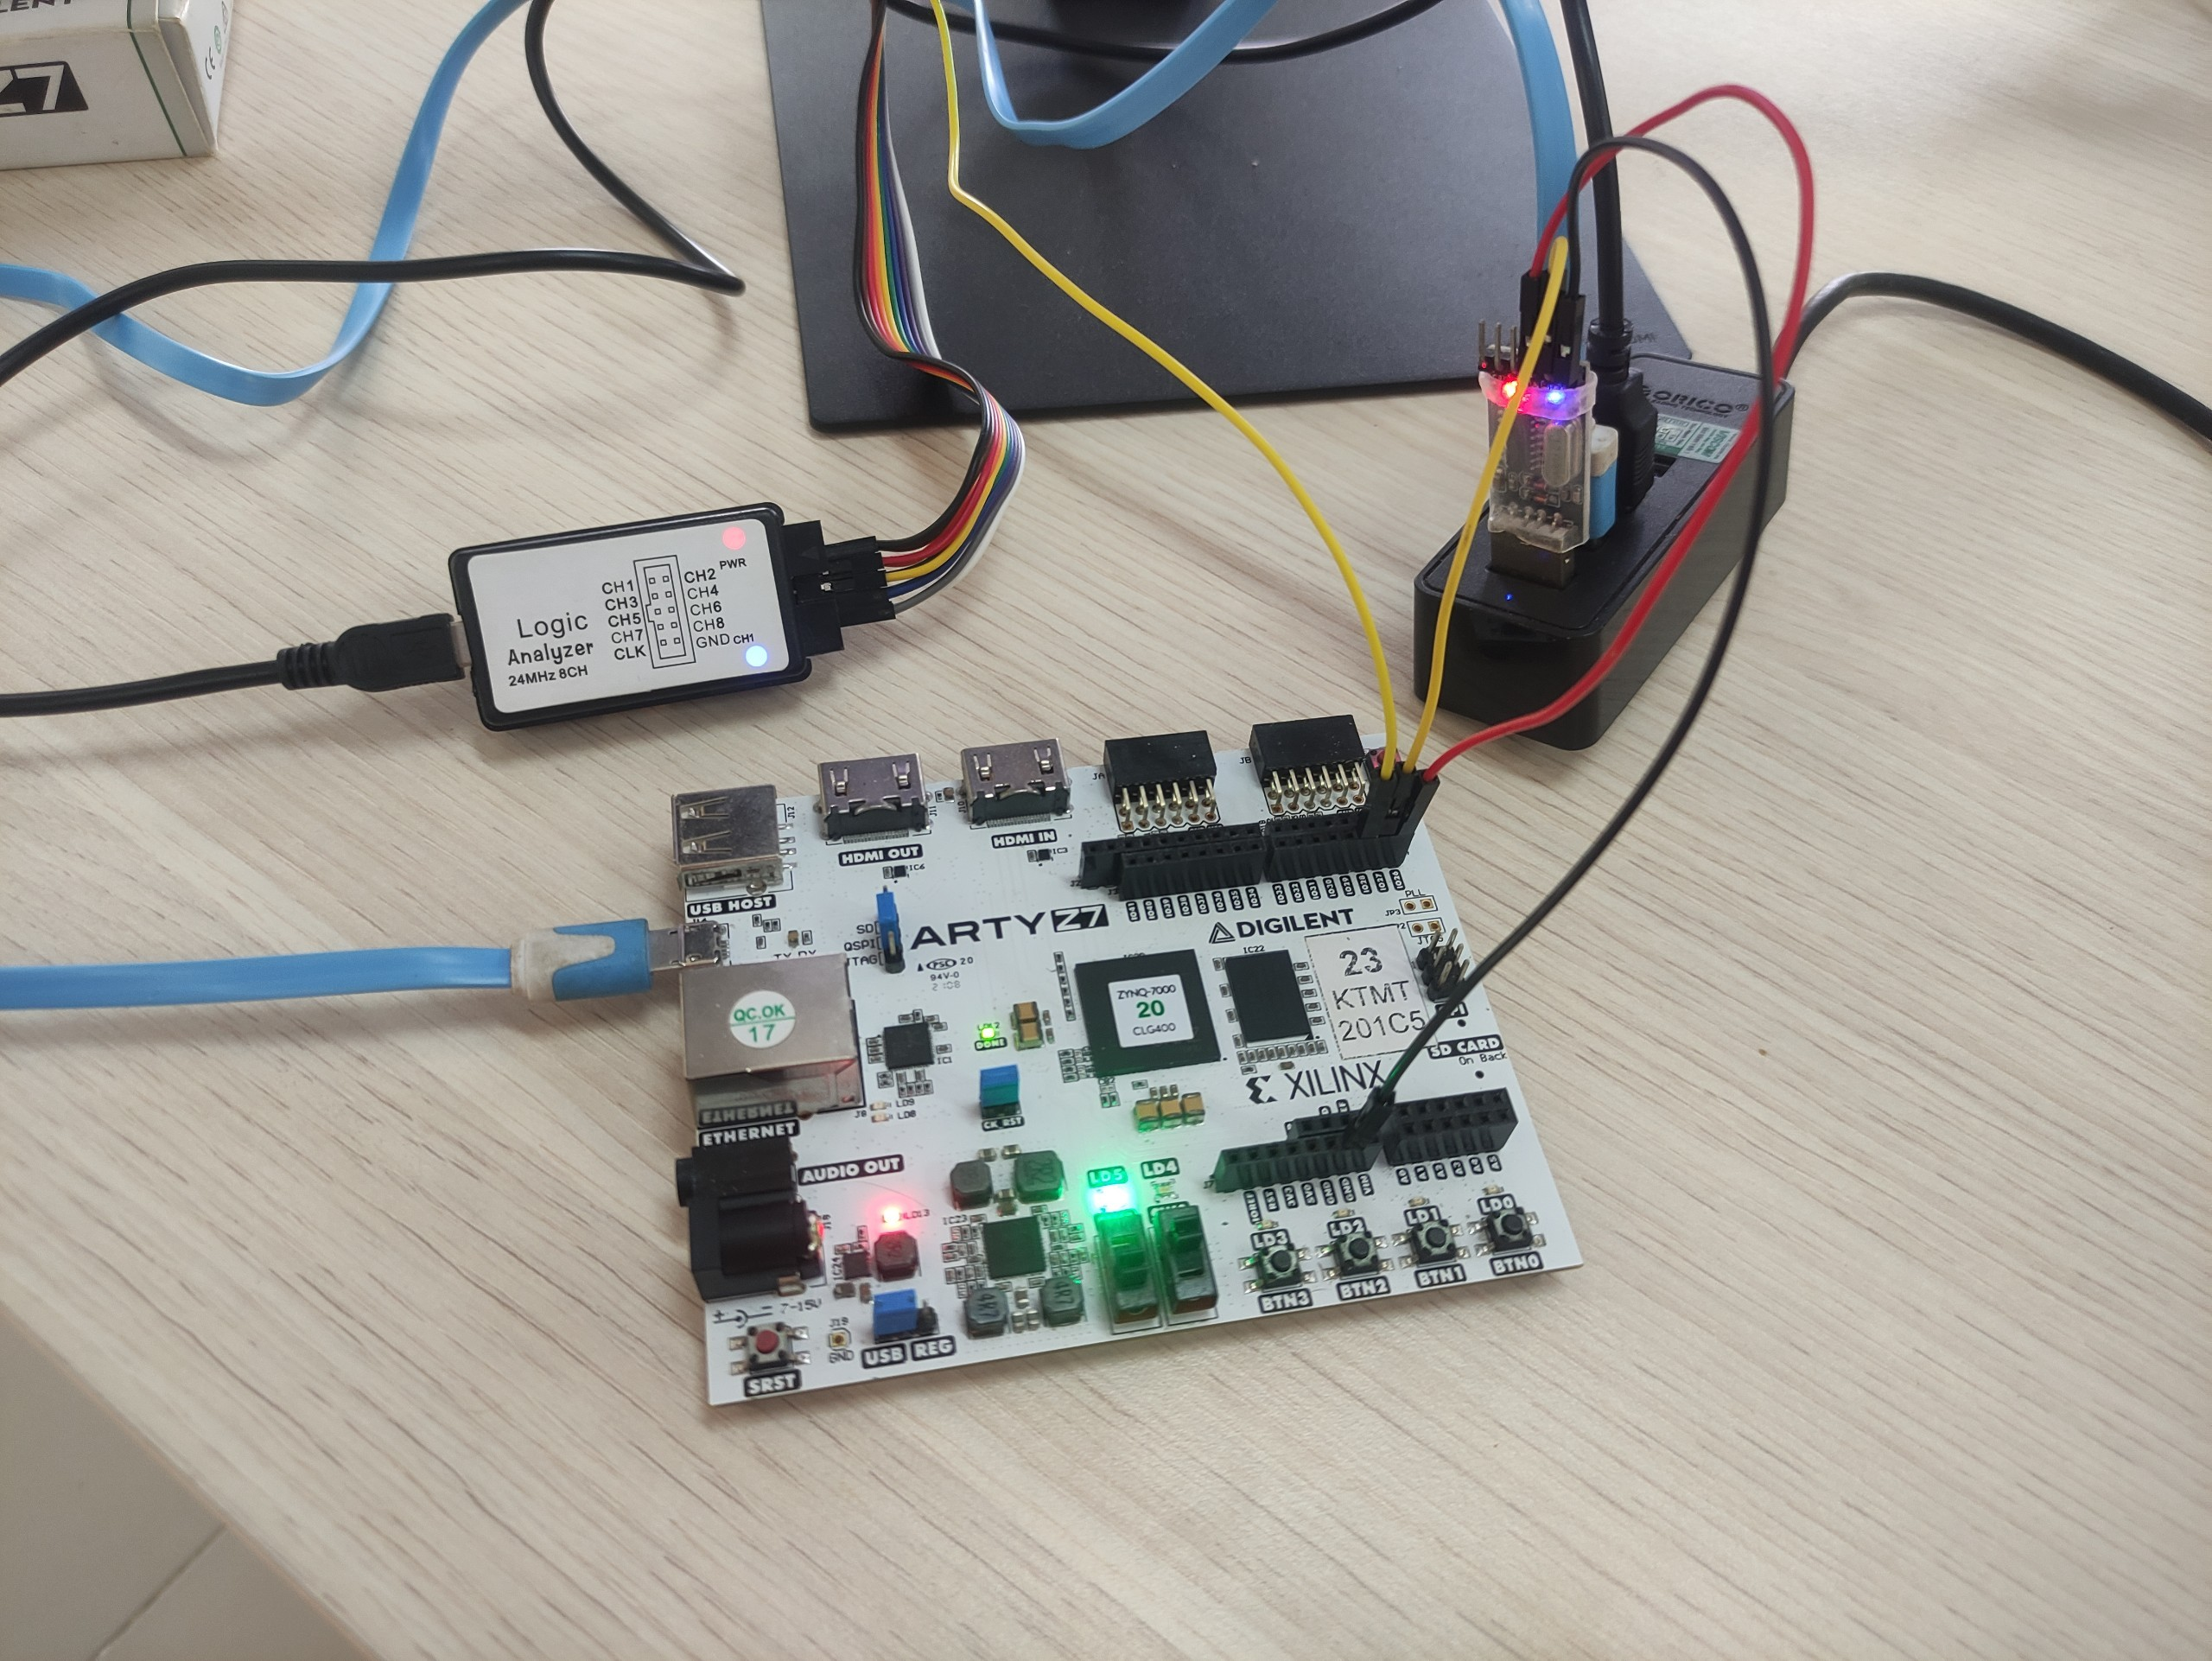
\includegraphics[width=0.9\linewidth]{2_co_so_ly_thuyet/image/uart.png} 
        \caption{Minh họa chân kết nối truyền nhận dữ liệu UART}
        \label{fig:uart_connection}
    \end{figure}

    \begin{figure}[H]
        \centering
        \includegraphics[width=0.8\linewidth]{2_co_so_ly_thuyet/image/uart2.png} 
        \caption{Chuyển đổi dữ liệu song song thành nối tiếp và ngược lại trong UART}
        \label{fig:uart_connection}
    \end{figure}



    \subsubsection{Cấu trúc khung dữ liệu (Data Frame)}
    Do không có xung nhịp đồng bộ, UART sử dụng các bit điều khiển đặc biệt để đánh dấu điểm bắt đầu và kết thúc của một gói tin. Một khung dữ liệu chuẩn bao gồm các thành phần sau:



    \begin{enumerate}
        \item \textbf{Trạng thái nghỉ (Idle State):} Khi không có dữ liệu truyền, đường truyền luôn được giữ ở mức điện áp cao (Logic 1).
        \item \textbf{Start Bit:} Để bắt đầu một phiên truyền, thiết bị phát sẽ kéo đường truyền từ mức cao xuống mức thấp (Logic 0) trong một chu kỳ bit. Bên thu phát hiện cạnh xuống này để bắt đầu quá trình đồng bộ.
        \item \textbf{Data Bits:} Chứa thông tin thực tế cần truyền, thường có độ dài từ 5 đến 9 bit (phổ biến nhất là 8 bit). Theo quy ước, bit có trọng số nhỏ nhất (LSB) được truyền đi trước.
        \item \textbf{Parity Bit (Tùy chọn):} Dùng để kiểm tra lỗi đơn giản. Bit này có thể được cấu hình là chẵn (Even), lẻ (Odd) hoặc không sử dụng (None). Nếu sử dụng, tổng số bit '1' trong gói dữ liệu (bao gồm cả parity) phải thỏa mãn quy tắc chẵn/lẻ đã thiết lập.
        \item \textbf{Stop Bit:} Đánh dấu kết thúc gói tin bằng cách kéo đường truyền về mức cao (Logic 1). Độ dài có thể là 1, 1.5, hoặc 2 bit thời gian. Stop bit đảm bảo đường truyền quay về trạng thái nghỉ để sẵn sàng cho Start bit tiếp theo.
    \end{enumerate}

    \begin{figure}[H]
        \centering
        \includegraphics[width=0.8\linewidth]{2_co_so_ly_thuyet/image/uart_frame.png} 
        \caption{Khung dữ liệu UART}
        \label{fig:uart_frame}
    \end{figure}

    \begin{figure}[H]
        \centering
        \includegraphics[width=0.8\linewidth]{2_co_so_ly_thuyet/image/uart_frame_example.png} 
        \caption{Ví dụ khung dữ liệu UART với 8bit dữ liệu, không parity và 1 stop bit}
        \label{fig:uart_frame}
    \end{figure}

    \subsubsection{Tốc độ Baud (Baud Rate)}
    Vì thiếu xung nhịp đồng bộ, hai thiết bị UART phải thống nhất trước một tốc độ truyền nhận, gọi là Baud Rate (đơn vị: bit/giây - bps).
    \begin{itemize}
        \item Bên phát sẽ đẩy từng bit dữ liệu ra đường truyền với chu kỳ $T = 1/BaudRate$.
        \item Bên thu sẽ lấy mẫu tín hiệu (sample) tại điểm giữa của mỗi chu kỳ bit dự kiến để đọc dữ liệu.
    \end{itemize}
    Theo khuyến cáo kỹ thuật, độ sai lệch tốc độ Baud giữa hai thiết bị không được vượt quá 10\% để đảm bảo dữ liệu được đọc chính xác. Các tốc độ phổ biến thường dùng là 9600, 19200, 115200 bps.


    \subsection{Giao thức truyền thông SPI}

SPI (Serial Peripheral Interface) là chuẩn giao tiếp nối tiếp đồng bộ tốc độ cao, hoạt động ở chế độ song công toàn phần (Full-duplex). Chuẩn này được Motorola giới thiệu vào giữa những năm 1980 và hiện nay đã trở thành tiêu chuẩn công nghiệp để kết nối vi xử lý với các thiết bị ngoại vi như cảm biến, bộ nhớ Flash (SPI Flash), màn hình LCD, hoặc bộ chuyển đổi ADC/DAC.

Khác với UART (bất đồng bộ) hay I2C (bán song công, tốc độ thấp), SPI sử dụng đường xung nhịp riêng biệt và kiến trúc Master-Slave chặt chẽ, cho phép đạt băng thông truyền tải rất cao (có thể lên tới hàng chục MHz).

\subsubsection{Cấu hình tín hiệu vật lý}
Một bus SPI tiêu chuẩn (4-wire mode) bao gồm 4 đường tín hiệu logic kết nối giữa Master và Slave.

% --- VỊ TRÍ CHÈN ẢNH 1: Sơ đồ kết nối Master-Slave ---
\begin{figure}[H]
    \centering
    % Bạn thay tên file ảnh vào dòng dưới
    \includegraphics[width=0.7\linewidth]{2_co_so_ly_thuyet/image/spiwrite.png} 
    \caption{Sơ đồ kết nối tín hiệu chuẩn 4 dây của SPI}
    \label{fig:spi_connection}
\end{figure}

Chức năng các chân tín hiệu bao gồm:
\begin{itemize}
    \item \textbf{SCLK (Serial Clock):} Tín hiệu xung nhịp do Master tạo ra. Toàn bộ quá trình truyền nhận dữ liệu được đồng bộ theo cạnh lên hoặc cạnh xuống của xung này. Slave không được phép tạo xung Clock.
    \item \textbf{MOSI (Master Out Slave In):} Đường truyền dữ liệu từ Master đến Slave.
    \item \textbf{MISO (Master In Slave Out):} Đường truyền dữ liệu từ Slave về Master. Nếu chỉ có Master gửi dữ liệu (ví dụ điều khiển LCD), chân này có thể bỏ qua.
    \item \textbf{CS/SS (Chip Select / Slave Select):} Tín hiệu chọn thiết bị, thường hoạt động ở mức thấp (Active Low). Master kéo chân này xuống 0V để bắt đầu giao dịch với một Slave cụ thể.
\end{itemize}

\subsubsection{Cơ chế hoạt động: Thanh ghi dịch (Shift Register)}
Cốt lõi của giao thức SPI là cấu trúc thanh ghi dịch vòng tròn (Circular Shift Register).

% --- VỊ TRÍ CHÈN ẢNH 2: Cơ chế thanh ghi dịch ---
\begin{figure}[H]
    \centering
    % Bạn thay tên file ảnh vào dòng dưới
    \includegraphics[width=0.9\linewidth]{2_co_so_ly_thuyet/image/spireg.png} 
    \caption{Cơ chế trao đổi dữ liệu dùng thanh ghi dịch trong SPI}
    \label{fig:spi_shift_register}
\end{figure}

Quá trình truyền nhận diễn ra như sau:
\begin{enumerate}
    \item Master và Slave mỗi bên đều có một thanh ghi dịch (thường là 8-bit hoặc 16-bit).
    \item Tại mỗi chu kỳ xung nhịp SCLK:
    \begin{itemize}
        \item 1 bit dữ liệu từ Master được đẩy ra đường MOSI và dịch vào thanh ghi của Slave.
        \item Đồng thời, 1 bit dữ liệu từ Slave được đẩy ra đường MISO và dịch vào thanh ghi của Master.
    \end{itemize}
    \item Sau $N$ chu kỳ xung nhịp (với $N$ là độ rộng dữ liệu), giá trị trong thanh ghi của Master và Slave được trao đổi hoàn toàn cho nhau.
    
\end{enumerate}

\subsubsection{Các chế độ hoạt động (Clock Polarity \& Phase)}
SPI định nghĩa 4 chế độ hoạt động (Modes) dựa trên trạng thái của xung Clock, được quy định bởi hai tham số:
\begin{itemize}
    \item \textbf{CPOL (Clock Polarity):} Trạng thái nghỉ của đường SCLK (0 hoặc 1).
    \item \textbf{CPHA (Clock Phase):} Cạnh lên hoặc xuống của xung dùng để lấy mẫu (Sample) và dùng để thay đổi dữ liệu (Shift).
\end{itemize}

% --- VỊ TRÍ CHÈN ẢNH 3: Giản đồ xung 4 Mode (Lấy từ file Analog Device) ---
% \begin{figure}[H]
%     \centering
%     % Bạn thay tên file ảnh vào dòng dưới
%     \includegraphics[width=0.9\linewidth]{2_co_so_ly_thuyet/image/spi_modes.png} 
%     \caption{Giản đồ thời gian của 4 chế độ hoạt động SPI (CPOL/CPHA)}
%     \label{fig:spi_modes}
% \end{figure}

\begin{figure}[H]
    \centering
    % Bạn thay tên file ảnh vào dòng dưới
    \includegraphics[width=1\linewidth]{2_co_so_ly_thuyet/image/spimode.png} 
    \caption{4 chế độ hoạt động của SPI(CPOL/CPHA)}
    \label{fig:spi_modes}
\end{figure}


\textit{Lưu ý:} Mode 0 và Mode 3 là hai cấu hình phổ biến nhất. Master và Slave phải được cấu hình cùng một Mode để giao tiếp thành công.

\begin{figure}[H]
    \centering
    % Bạn thay tên file ảnh vào dòng dưới
    \includegraphics[width=1\linewidth]{2_co_so_ly_thuyet/image/spimod0.png} 
    \caption{SPI MODE 0 (CPOL=0, CPHA=0), trạng thái SCLK ban đầu ở mức low, dữ liệu được lấy mẫu tại cạnh lên của SCLK và dịch ở cạnh xuống}
    \label{fig:spi_modes}
\end{figure}

\begin{figure}[H]
    \centering
    % Bạn thay tên file ảnh vào dòng dưới
    \includegraphics[width=1\linewidth]{2_co_so_ly_thuyet/image/spimode3.png} 
    \caption{SPI MODE 3 (CPOL=1, CPHA=1), trạng thái SCLK ban đầu ở mức high, dữ liệu được lấy mẫu tại cạnh lên của SCLK và dịch ở cạnh xuống}
    \label{fig:spi_modes}
\end{figure}

\subsubsection{Các mô hình kết nối đa thiết bị}
SPI cho phép một Master giao tiếp với nhiều Slave thông qua hai cấu hình chính:

\textbf{1. Cấu hình Slave độc lập (Independent Slaves):} \\
Master sử dụng các chân CS riêng biệt ($CS_1, CS_2, ...$) cho từng Slave. Đây là cấu hình phổ biến giúp tối ưu băng thông.

\begin{figure}[H]
    \centering
    % Bạn thay tên file ảnh vào dòng dưới
    \includegraphics[width=0.9\linewidth]{2_co_so_ly_thuyet/image/spisingle.png} 
    \caption{Cấu hình Slave độc lập trong SPI}
    \label{fig:spi_modes}
\end{figure}

\textbf{2. Cấu hình Chuỗi (Daisy Chain):} \\
Các Slave được nối tiếp nhau (MISO của Slave này nối vào MOSI của Slave kia). Dữ liệu đi qua chuỗi các thiết bị, giúp tiết kiệm chân điều khiển của Master nhưng làm giảm tốc độ truyền tổng thể.

\begin{figure}[H]
    \centering
    % Bạn thay tên file ảnh vào dòng dưới
    \includegraphics[width=0.9\linewidth]{2_co_so_ly_thuyet/image/spidaisy.png} 
    \caption{Cấu hình Chuỗi (Daisy Chain) trong SPI}
    \label{fig:spi_modes}
\end{figure}

% --- VỊ TRÍ CHÈN ẢNH 4: Cấu hình Daisy Chain vs Independent ---
% \begin{figure}[H]
%     \centering
%     % Bạn thay tên file ảnh vào dòng dưới
%     \includegraphics[width=0.8\linewidth]{2_co_so_ly_thuyet/image/spi_configs.png} 
%     \caption{Hai mô hình kết nối đa thiết bị trong SPI: Độc lập và Chuỗi}
%     \label{fig:spi_configs}
% \end{figure}


    SPI có tốc độ truyền cao nhất so với UART và I2C, phần cứng đơn giản, hỗ trợ Full-duplex. Nhưng tốn nhiều dây tín hiệu, khoảng cách truyền ngắn, không có cơ chế xác nhận lỗi (ACK) như I2C.
